% CogFormer — Decoder (flow-matching velocity field over parameter tokens)
% Literal computational block diagram. Compile standalone:
%   pdflatex cogformer_decoder.tex
\documentclass[border=8pt]{standalone}
\usepackage{amsmath}
\usepackage{amssymb}
\usepackage{tikz}
\usetikzlibrary{arrows.meta, positioning, fit, backgrounds, calc}

\begin{document}
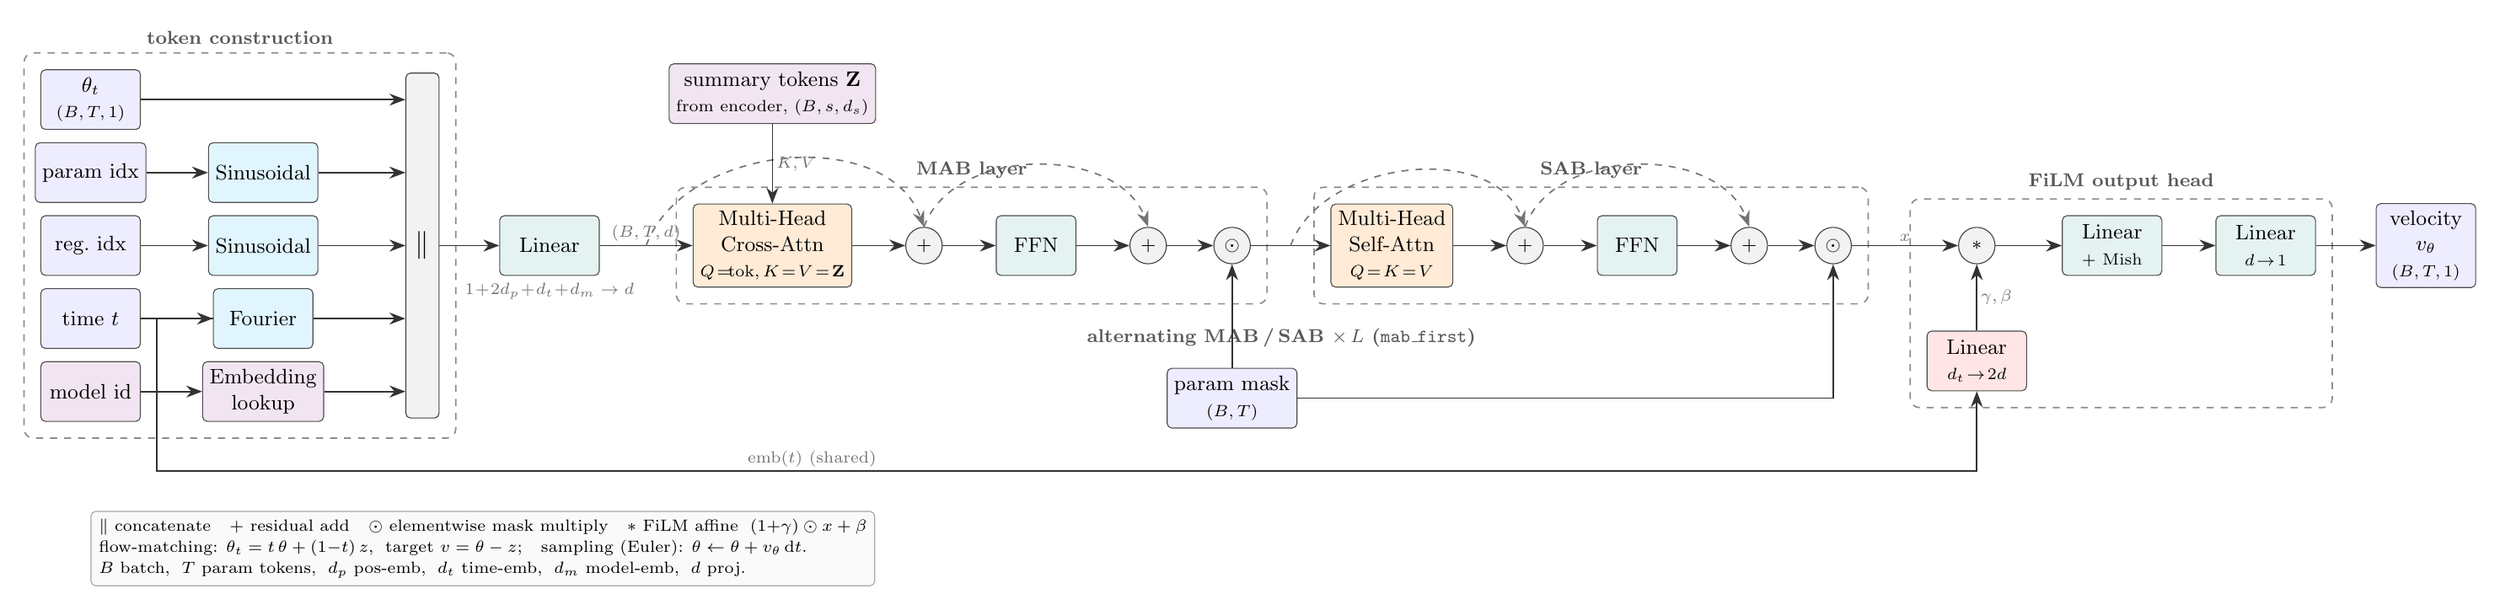
\begin{tikzpicture}[
  font=\small,
  node distance=8mm,
  >={Stealth[length=2.4mm]},
  block/.style={rounded corners=2pt, draw=black!70, fill=#1,
                minimum height=9mm, minimum width=15mm, align=center, inner sep=3pt},
  block/.default=white,
  data/.style={block=blue!7},
  emb/.style={block=cyan!12},
  lin/.style={block=teal!10},
  attn/.style={block=orange!16, minimum height=12mm},
  film/.style={block=red!10},
  ctx/.style={block=violet!10},
  op/.style={circle, draw=black!75, fill=black!5, inner sep=0pt,
             minimum size=5.5mm, font=\footnotesize},
  bus/.style={draw=black!75, fill=black!5, rounded corners=2pt,
              minimum width=5mm, minimum height=52mm, font=\large},
  grp/.style={rounded corners=4pt, draw=black!45, dashed, line width=0.6pt, inner sep=7pt},
  grplab/.style={font=\footnotesize\bfseries, text=black!65},
  flow/.style={->, semithick, draw=black!80},
  res/.style={->, semithick, draw=black!55, dashed},
  shp/.style={font=\scriptsize, text=black!55, inner sep=1.5pt},
]

% ======================= INPUTS =======================
\node[data] (theta) at (0, 2.2) {$\theta_t$\\{\scriptsize$(B,T,1)$}};
\node[data] (pidx)  at (0, 1.1) {param idx};
\node[data] (ridx)  at (0, 0.0) {reg.\ idx};
\node[data] (tval)  at (0,-1.1) {time $t$};
\node[ctx]  (mid)   at (0,-2.2) {model id};

% ---- per-scalar embeddings ----
\node[emb] (psin) at (2.6, 1.1) {Sinusoidal};
\node[emb] (rsin) at (2.6, 0.0) {Sinusoidal};
\node[emb] (tfou) at (2.6,-1.1) {Fourier};
\node[ctx] (memb) at (2.6,-2.2) {Embedding\\lookup};
\draw[flow] (pidx) -- (psin);
\draw[flow] (ridx) -- (rsin);
\draw[flow] (tval) -- (tfou);
\draw[flow] (mid)  -- (memb);

% ---- concat "bus" ----
\node[bus] (cat) at (5.0,0) {$\Vert$};
\draw[flow] (theta) -- (cat.west |- theta);
\draw[flow] (psin)  -- (cat.west |- psin);
\draw[flow] (rsin)  -- (cat.west |- rsin);
\draw[flow] (tfou)  -- (cat.west |- tfou);
\draw[flow] (memb)  -- (cat.west |- memb);

\node[lin, right=9mm of cat] (iproj) {Linear};
\draw[flow] (cat.east) -- (iproj);
\node[shp, below=0.5mm of iproj] {$1\!+\!2d_p\!+\!d_t\!+\!d_m \to d$};

\begin{scope}[on background layer]
  \node[grp, fit=(theta)(mid)(psin)(memb)(cat),
        label={[grplab]above:token construction}] {};
\end{scope}

% ======================= MIXED ATTENTION STACK =======================
% Layer (odd): MAB — cross-attention to encoder summary tokens Z
\node[attn, right=14mm of iproj] (mab) {Multi-Head\\Cross-Attn\\{\scriptsize$Q\!=\!$tok,\,$K\!=\!V\!=\!\mathbf{Z}$}};
\node[op,   right=of mab]        (m1)  {$+$};
\node[lin,  right=of m1, minimum width=12mm] (mffn) {FFN};
\node[op,   right=of mffn]       (m2)  {$+$};
\node[op,   right=7mm of m2]     (mmask){$\odot$};

% Layer (even): SAB — self-attention among parameter tokens
\node[attn, right=12mm of mmask] (sab) {Multi-Head\\Self-Attn\\{\scriptsize$Q\!=\!K\!=\!V$}};
\node[op,   right=of sab]        (s1)  {$+$};
\node[lin,  right=of s1, minimum width=12mm] (sffn) {FFN};
\node[op,   right=of sffn]       (s2)  {$+$};
\node[op,   right=7mm of s2]     (smask){$\odot$};

\draw[flow] (iproj) -- (mab) node[shp, midway, above]{$(B,T,d)$};
\draw[flow] (mab) -- (m1);
\draw[flow] (m1)  -- (mffn);
\draw[flow] (mffn)-- (m2);
\draw[flow] (m2)  -- (mmask);
\draw[flow] (mmask)-- (sab);
\draw[flow] (sab) -- (s1);
\draw[flow] (s1)  -- (sffn);
\draw[flow] (sffn)-- (s2);
\draw[flow] (s2)  -- (smask);

% residual adds (pre-LN inside each MAB/SAB; LN omitted for compactness)
\coordinate (mtap) at ($(iproj.east)!0.5!(mab.west)$);
\draw[res] (mtap) to[out=70,in=110] (m1.north);
\draw[res] (m1.north) to[out=70,in=110] (m2.north);
\coordinate (stap) at ($(mmask.east)!0.5!(sab.west)$);
\draw[res] (stap) to[out=70,in=110] (s1.north);
\draw[res] (s1.north) to[out=70,in=110] (s2.north);

% encoder summary tokens Z -> cross-attention K,V
\node[ctx, above=12mm of mab] (Z) {summary tokens $\mathbf{Z}$\\{\scriptsize from encoder, $(B,s,d_s)$}};
\draw[flow] (Z) -- (mab) node[shp, midway, right]{$K,V$};

\begin{scope}[on background layer]
  \node[grp, fit=(mab)(m1)(mffn)(m2)(mmask),
        label={[grplab]above:MAB layer}] (mabg) {};
  \node[grp, fit=(sab)(s1)(sffn)(s2)(smask),
        label={[grplab]above:SAB layer}] (sabg) {};
\end{scope}
\node[grplab] at ($(mabg.south)!0.5!(sabg.south)+(0,-0.5)$)
      {alternating MAB\,/\,SAB $\times\,L$ (\texttt{mab\_first})};

% ======================= FiLM OUTPUT HEAD =======================
\node[op,   right=16mm of smask]              (filmop) {$*$};
\node[film, below=10mm of filmop]             (filmproj){Linear\\{\scriptsize$d_t\!\to\!2d$}};
\node[lin,  right=10mm of filmop]             (h)   {Linear\\{\scriptsize+ Mish}};
\node[lin,  right=of h]                        (out) {Linear\\{\scriptsize$d\!\to\!1$}};
\node[data, right=9mm of out]                  (v)   {velocity\\$v_\theta$\\{\scriptsize$(B,T,1)$}};

\draw[flow] (smask) -- (filmop) node[shp, midway, above]{$x$};
\draw[flow] (filmproj) -- (filmop) node[shp, midway, right]{$\gamma,\beta$};
\draw[flow] (filmop) -- (h);
\draw[flow] (h) -- (out);
\draw[flow] (out) -- (v);

\begin{scope}[on background layer]
  \node[grp, fit=(filmop)(filmproj)(h)(out),
        label={[grplab]above:FiLM output head}] {};
\end{scope}

% ======================= BOTTOM RAILS =======================
% parameter mask -> both elementwise mask multiplies
\node[data] (pmask) at (mmask |- 0,-2.3) {param mask\\{\scriptsize$(B,T)$}};
\draw[flow] (pmask) -- (mmask);
\draw[flow] (pmask.east) -| (smask);

% time embedding reused by FiLM: routed left of the inputs, then along the bottom
\draw[flow] (tfou.west) -- (1.0,-1.1) -- (1.0,-3.4) -| (filmproj.south)
      node[shp, pos=0.18, above]{$\mathrm{emb}(t)$ (shared)};

% ======================= LEGEND =======================
\node[draw=black!35, rounded corners=2pt, fill=black!2, align=left,
      font=\scriptsize, anchor=north west] at (0,-4.0)
  {$\Vert$ concatenate\quad $+$ residual add\quad
   $\odot$ elementwise mask multiply\quad
   $*$ FiLM affine $\;(1{+}\gamma)\odot x+\beta$\\[1pt]
   flow-matching: $\theta_t=t\,\theta+(1{-}t)\,z$,\; target $v=\theta-z$;\quad
   sampling (Euler): $\theta\leftarrow\theta+v_\theta\,\mathrm{d}t$.\\[1pt]
   $B$ batch,\; $T$ param tokens,\; $d_p$ pos-emb,\; $d_t$ time-emb,\; $d_m$ model-emb,\; $d$ proj.};

\end{tikzpicture}
\end{document}
